\documentclass[10.5pt]{ctexart}
\usepackage{graphicx}
\usepackage{indentfirst}
\usepackage[a4paper, inner=1.5cm, outer=3cm, top=2cm, bottom=3cm, bindingoffset=1cm]{geometry}
\usepackage{array}
\usepackage{fontspec}
\usepackage{gensymb}
\usepackage{makecell}
\usepackage[lofdepth,lotdepth]{subfig}
\setlength{\extrarowheight}{4pt}
\begin{document}
\title{\textbf{\fontsize{15.75pt}{\baselineskip}{常用电子仪器的原理与使用实验报告}}} % 15.75pt is 3 号 in chinese
\author{\fontsize{12pt}{\baselineskip}{数33 赵丰 2013012178}}
\date{\fontsize{12pt}{\baselineskip}{9 21,2016}}
\maketitle
\section{\textbf{\fontsize{12pt}{\baselineskip}{引言}}}
常用电子仪器是电子学实验的基本设备,正确使用常用电子仪器是做实验的基本条件。本次实验将使用Agilent数字示波器
TFG函数信号发生器进行简单的测量。
\section{\textbf{\fontsize{12pt}{\baselineskip}{实验操作}}}
\begin{enumerate}
\item 示波器和函数信号发生器的应用
\begin{enumerate}
\item 观察示波器的校准信号
\item 用示波器测量函数信号发生器输出的正弦交流电压的幅度、周期和频率。
\item 测量一二端网络在不同频率输入电压下的输出电压的有效值和相位差。
\item 测量函数信号发生器输出方波的幅度、频率和占空比等参数。
\item 测量方波信号的上升沿和下降沿。
\item 示波器探头对测量结果的影响。
\item 示波器测量直流电压。
\end{enumerate}
\item 二端口网路参数的测量
\item 三极管9011 $\beta$值的测量
\end{enumerate}
\section{\textbf{\fontsize{12pt}{\baselineskip}{结果与讨论}}}
1(a)\quad 示波器接Demo 2信号源在X1衰减、直流耦合的情况下波形图Figure 1如下所示:
\newpage
\begin{figure}[!ht]
\centering
\caption{示波器校准信号波形图}
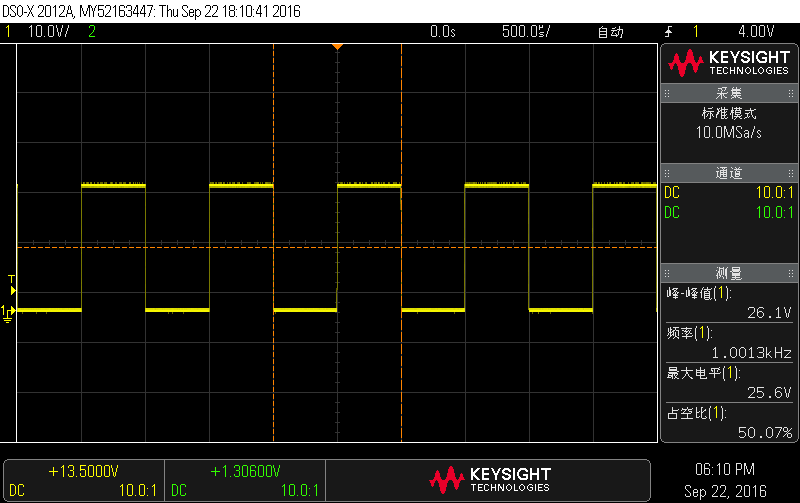
\includegraphics[width=350pt]{image/CalibratingSignal.png}
\end{figure}
若将探头改为X10衰减,则测得的方波高低电平分别为$\pm$2.57V。

1(b)\quad 测得的正弦交流信号如下Figure 2所示:
\begin{figure}[!ht]
\centering
\caption{正弦交流信号波形图}
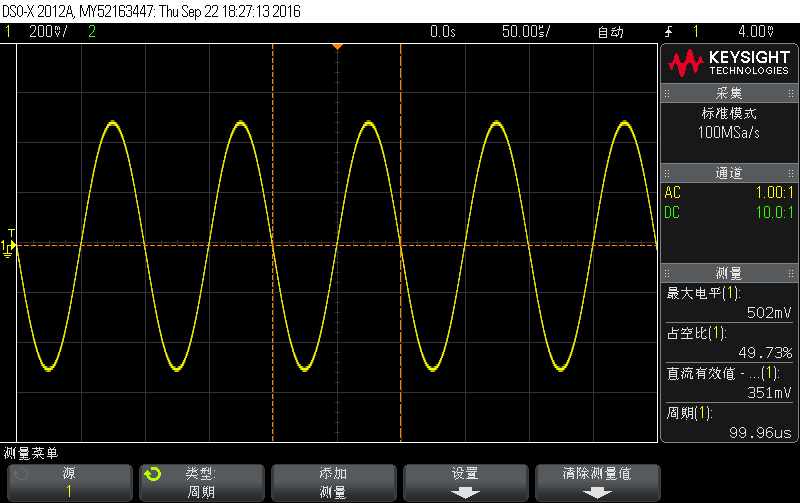
\includegraphics[width=350pt]{image/SineWave.png}
\end{figure}

1(c)用相量法对该二端网络进行求解,得到输出电压有效值$U_o$与输入电压$U_i$之间的关系为:
\begin{equation}
U_o=U_i \frac{j \omega C_1}{j \omega (C_1+2C_2) +\frac{1}{R1}-\omega_2 C_1 C_2 R_2}
\end{equation}
通过对上式代入元件参数和用示波器实际测量得到的结果如下表所示:
\begin{table}[!ht]
\centering
\caption{$U_o$的有效值和相位差}
\begin{tabular}{ccccc}
\hline
频率(kHz) & 理论有效值(mV) & 实测有效值(mV) & 理论相位差(rad) & 实测相位差(rad) \\
\hline
10 & 588 & 579 & -0.57 & -0.62 \\
20 & 435 & 417 & -0.91 & -0.93 \\
\hline
\end{tabular}
\end{table}

上图Figure 3是f=10kHz时输入信号波形与输出信号波形的截图:
\begin{figure}
\centering
\caption{f=10kHz时输入信号波形与输出信号波形}
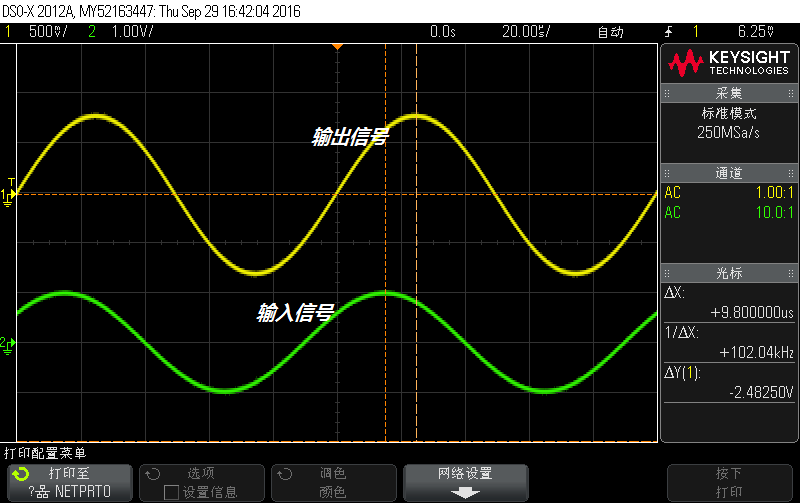
\includegraphics[width=350pt]{image/InputSignalWaveFormAndOutputSignalWaveForm.png}
\end{figure}


1(d)用示波器测量函数信号发生器在不同占空比下的方波波形,结果如下表所示:
\begin{table}[!ht]
\centering
\caption{$U_o$的有效值和相位差}
\begin{tabular}{ccccc}
\hline
 &信号发生器示值& D=50\% & D=99.9\% & D=0.1\%  \\
\hline
幅度(V) & 2.5 &2.49 & 2.49 & 2.49  \\
周期(ms) & 1 & 1 & 1 & 1  \\
频率(kHz) & 1 & 1 & 1 & 1  \\
占空比测量值(\%) & & 50 & 99.9 & 0.1\\
最大电平(V) & & 1.33& 40 &2.53\\
最小电平(V) & & -1.33 & -2.53 & -40m \\
\hline
\end{tabular}
\end{table}

1(e) 该RC网络虽然是一个二阶系统,但两个特征值的量阶相差1000倍,应以时间常数小的为参考,于是可将该网络看作一个一阶系统,时间常数$\tau =0.01ms$,对给定的方波输入信号,$T=0.2ms$,因此在半个周期可认为系统可达到稳态。根据上升时间和下降时间的定义,可求出$t_r=t_f=22\mu s$.实际测量结果为$t_r=23.5\mu s,t_f=24.6\mu s$

下图Figure 4是f=5kHz的输入方波信号波形与输出信号波形的截图:
\newpage
\begin{figure}[!ht]
\centering
\caption{f=10kHz时输入方波信号波形与输出信号波形}
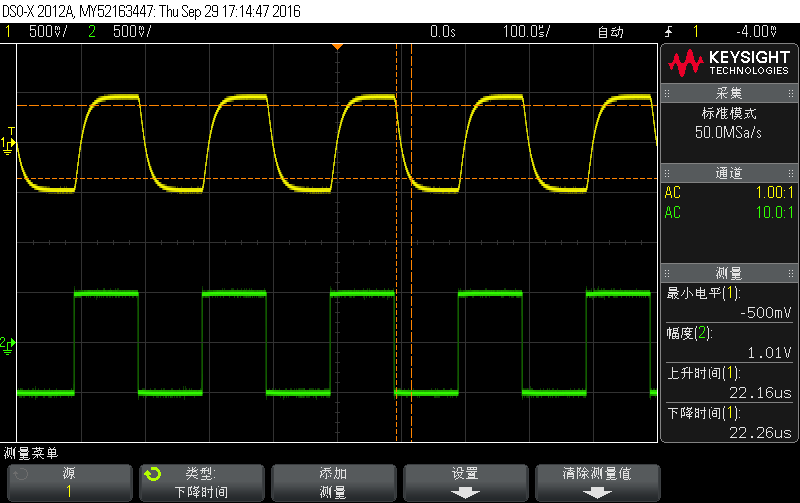
\includegraphics[width=350pt]{image/SquareWaveSignalInputAndOutputSignalWaveForm.png}
\end{figure}
1(f)对给定的电阻分压网络测定输出电压,理论值为500mV,下表给出了用不同的示波器探头对不同频率的正弦信号
的测量结果:
\begin{table}[!ht]
\centering
\caption{不同的示波器探头对测量结果的影响(单位:mV)}
\begin{tabular}{c|cc}
\hline
\diaghead{aaaaaaaaaaaaa}{input signal}{探头} & $\times$ 1 & $\times$ 10 \\
\hline
100kHz & 510 & 530  \\
400kHz & 430 & 530  \\
\hline
\end{tabular}
\end{table}

由上表可见,测量高频信号时,应用10X的探头。

1(g) 对电阻分压网络的输入端加12V直流电压,用示波器(直流耦合)测得的输入电压为12.1V,输出电压为6.4V,
而理论输出电压为6V。


2对给定的RC网络,输出端开路,输入电阻可由RC元件串并联关系得到;输入端开路,输出电阻也可由RC元件串并联关系得到。
测量时在输入端串入一个与理论值阻值接近的电阻(5100 $\Omega$),
由分压关系可间接测出输入电阻。输出电阻可利用Th\'evenin's Theorem间接测出。下表Table 4为理论值与实测值的对比:
\begin{table}[!ht]
\centering
\caption{RC网络输入与输出电阻测量(单位:$\Omega$)}
\begin{tabular}{cc|cc}
\hline
理论输入电阻 & 5081 & 理论输出电阻 & 5087  \\
\hline
实测输入电阻 & 5242 & 实测输出电阻 & 5100  \\
\hline
\end{tabular}
\end{table}

利用式(1),可得出$|\frac{U_o}{U_i}|~omega$的理论幅频特征曲线,再换算成关于f即可。
实际测量时,参考理论求出的$f_L,f_H$采用逐点法进行测量。
下图是理论曲线与实测曲线的对比:
\newpage
\begin{figure}[!ht]
\centering
\caption{RC网络幅频特征曲线}
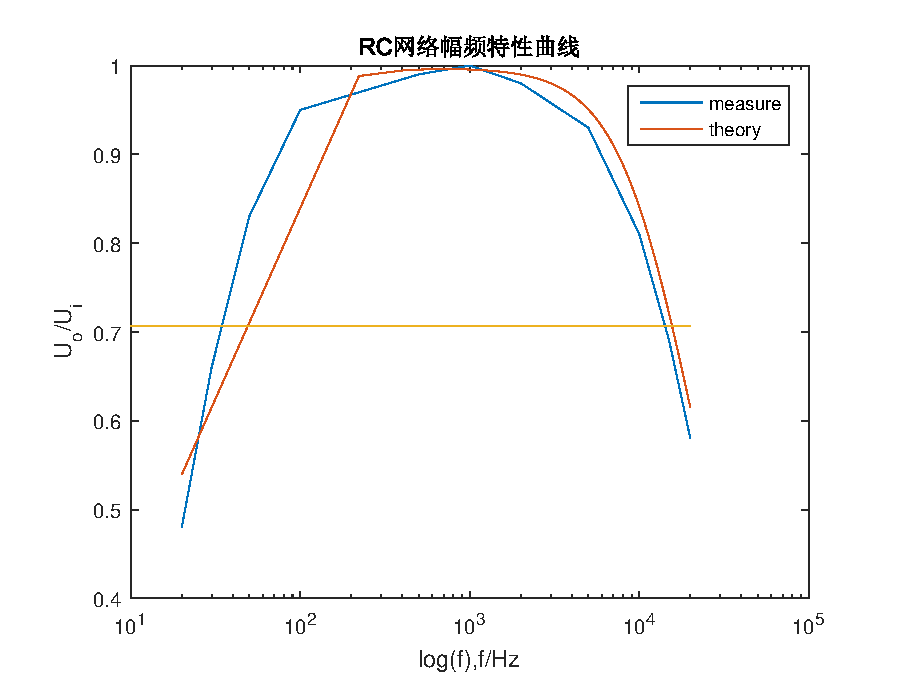
\includegraphics[width=400pt]{image/amplitudeFrequencyCharacteristics.eps}
\end{figure}
利用插值的方法可求得实测上下限截止频率,下表Table 5为理论值与实测值的对比:
\begin{table}[!ht]
\centering
\caption{RC网络上下限截止频率}
\begin{tabular}{cccc}
\hline
 & $f_L$ & $f_H$ & $\Delta$ f \\
\hline
理论& 31 & 1.56E4 &  1.56E4  \\
实测& 34 & 1.43E4 &  1.43E4  \\
\hline
\end{tabular}
\end{table}

3利用示波器的X-Y工作方式测定9011三极管的输出特性曲线如下图Figure 6所示,
其中横轴为$U_{CE}/V$,纵轴为$I_C$1V代表1mA。
\newpage
\begin{figure}[!ht]
\centering
\caption{三极管的输出特性曲线}
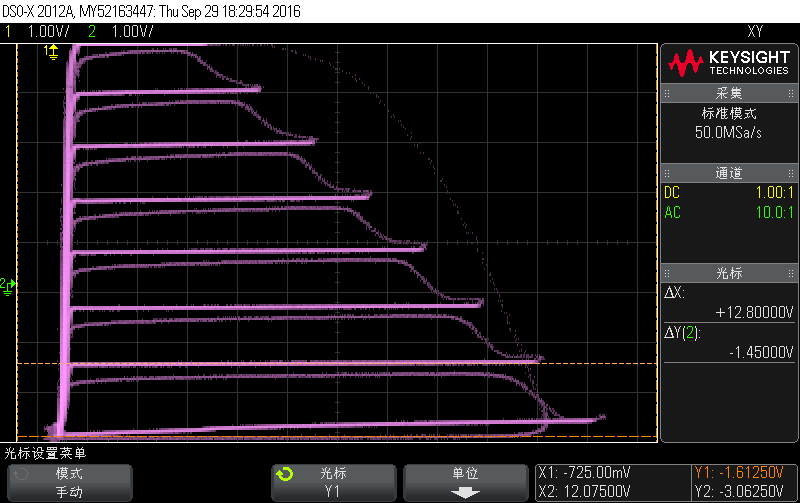
\includegraphics[width=350pt]{image/outputOfTransistor.png}
\end{figure}
利用示波器的光标可读出不同$I_B$下的$I_C$,进而求出放大倍数,结果如下表Table 6所示:
\begin{table}[!ht]
\centering
\caption{三极管输入电流与放大倍数}
\begin{tabular}{ccc}
\hline
$I_B(\mu A)$ & $I_C(mA)$ & $\beta$ \\
\hline
 5 & 1.45 &  290  \\
 10 & 2.54 &  254  \\
\hline
\end{tabular}
\end{table}


\section{\textbf{\fontsize{12pt}{\baselineskip}{参考文献}}}
\begin{thebibliography}{}
\bibitem{Bib1}电工技术与电子技术(上、下册) \quad 清华大学出版社
\end{thebibliography}
\end{document}